\documentclass[a4paper,11pt]{article}


\usepackage{amsmath,amsfonts,amsthm,a4wide}
\usepackage{graphicx}
\usepackage[super]{nth}
\usepackage{mathtools}


\begin{document}
\begin{center}
University of Toronto at Scarborough\\[0.1in]
{\bf CSCC73H3 Algorithm Design and Analysis, FALL 2018} \\[0.1in]
{\large{\bf Assignment No.5.Q1: Dynamic Programming and Network Flow}}\\[0.1in]
{\bf DUE:} November 15, 2018, at 11:59 pm
\end{center}


\vspace{0.1in}
\noindent
{\bf Student ID:} 1005642654 \\[0.15in]
{\bf Student Name:} KyooSik Lee
\vspace{0.3in}

\vspace{0.3in}
\begin{enumerate}

\item {\bf description}

My algorithm uses the algorithm that was used in the class. 

Using dynamic programming, I will work on the small problems first and then the big one.

My algorithm will store for each possible root, the total number of node in that tree without the root. So for the following figure, the number stored will be 2.

\begin{figure}[hbt]
	\centering
	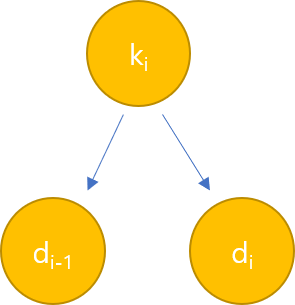
\includegraphics[scale=0.4]{figure1.png}
	\caption{Basic Tree}
\end{figure}

And we will use the same table (45 degree tilted table).

\begin{figure}[hbt]
	\centering
	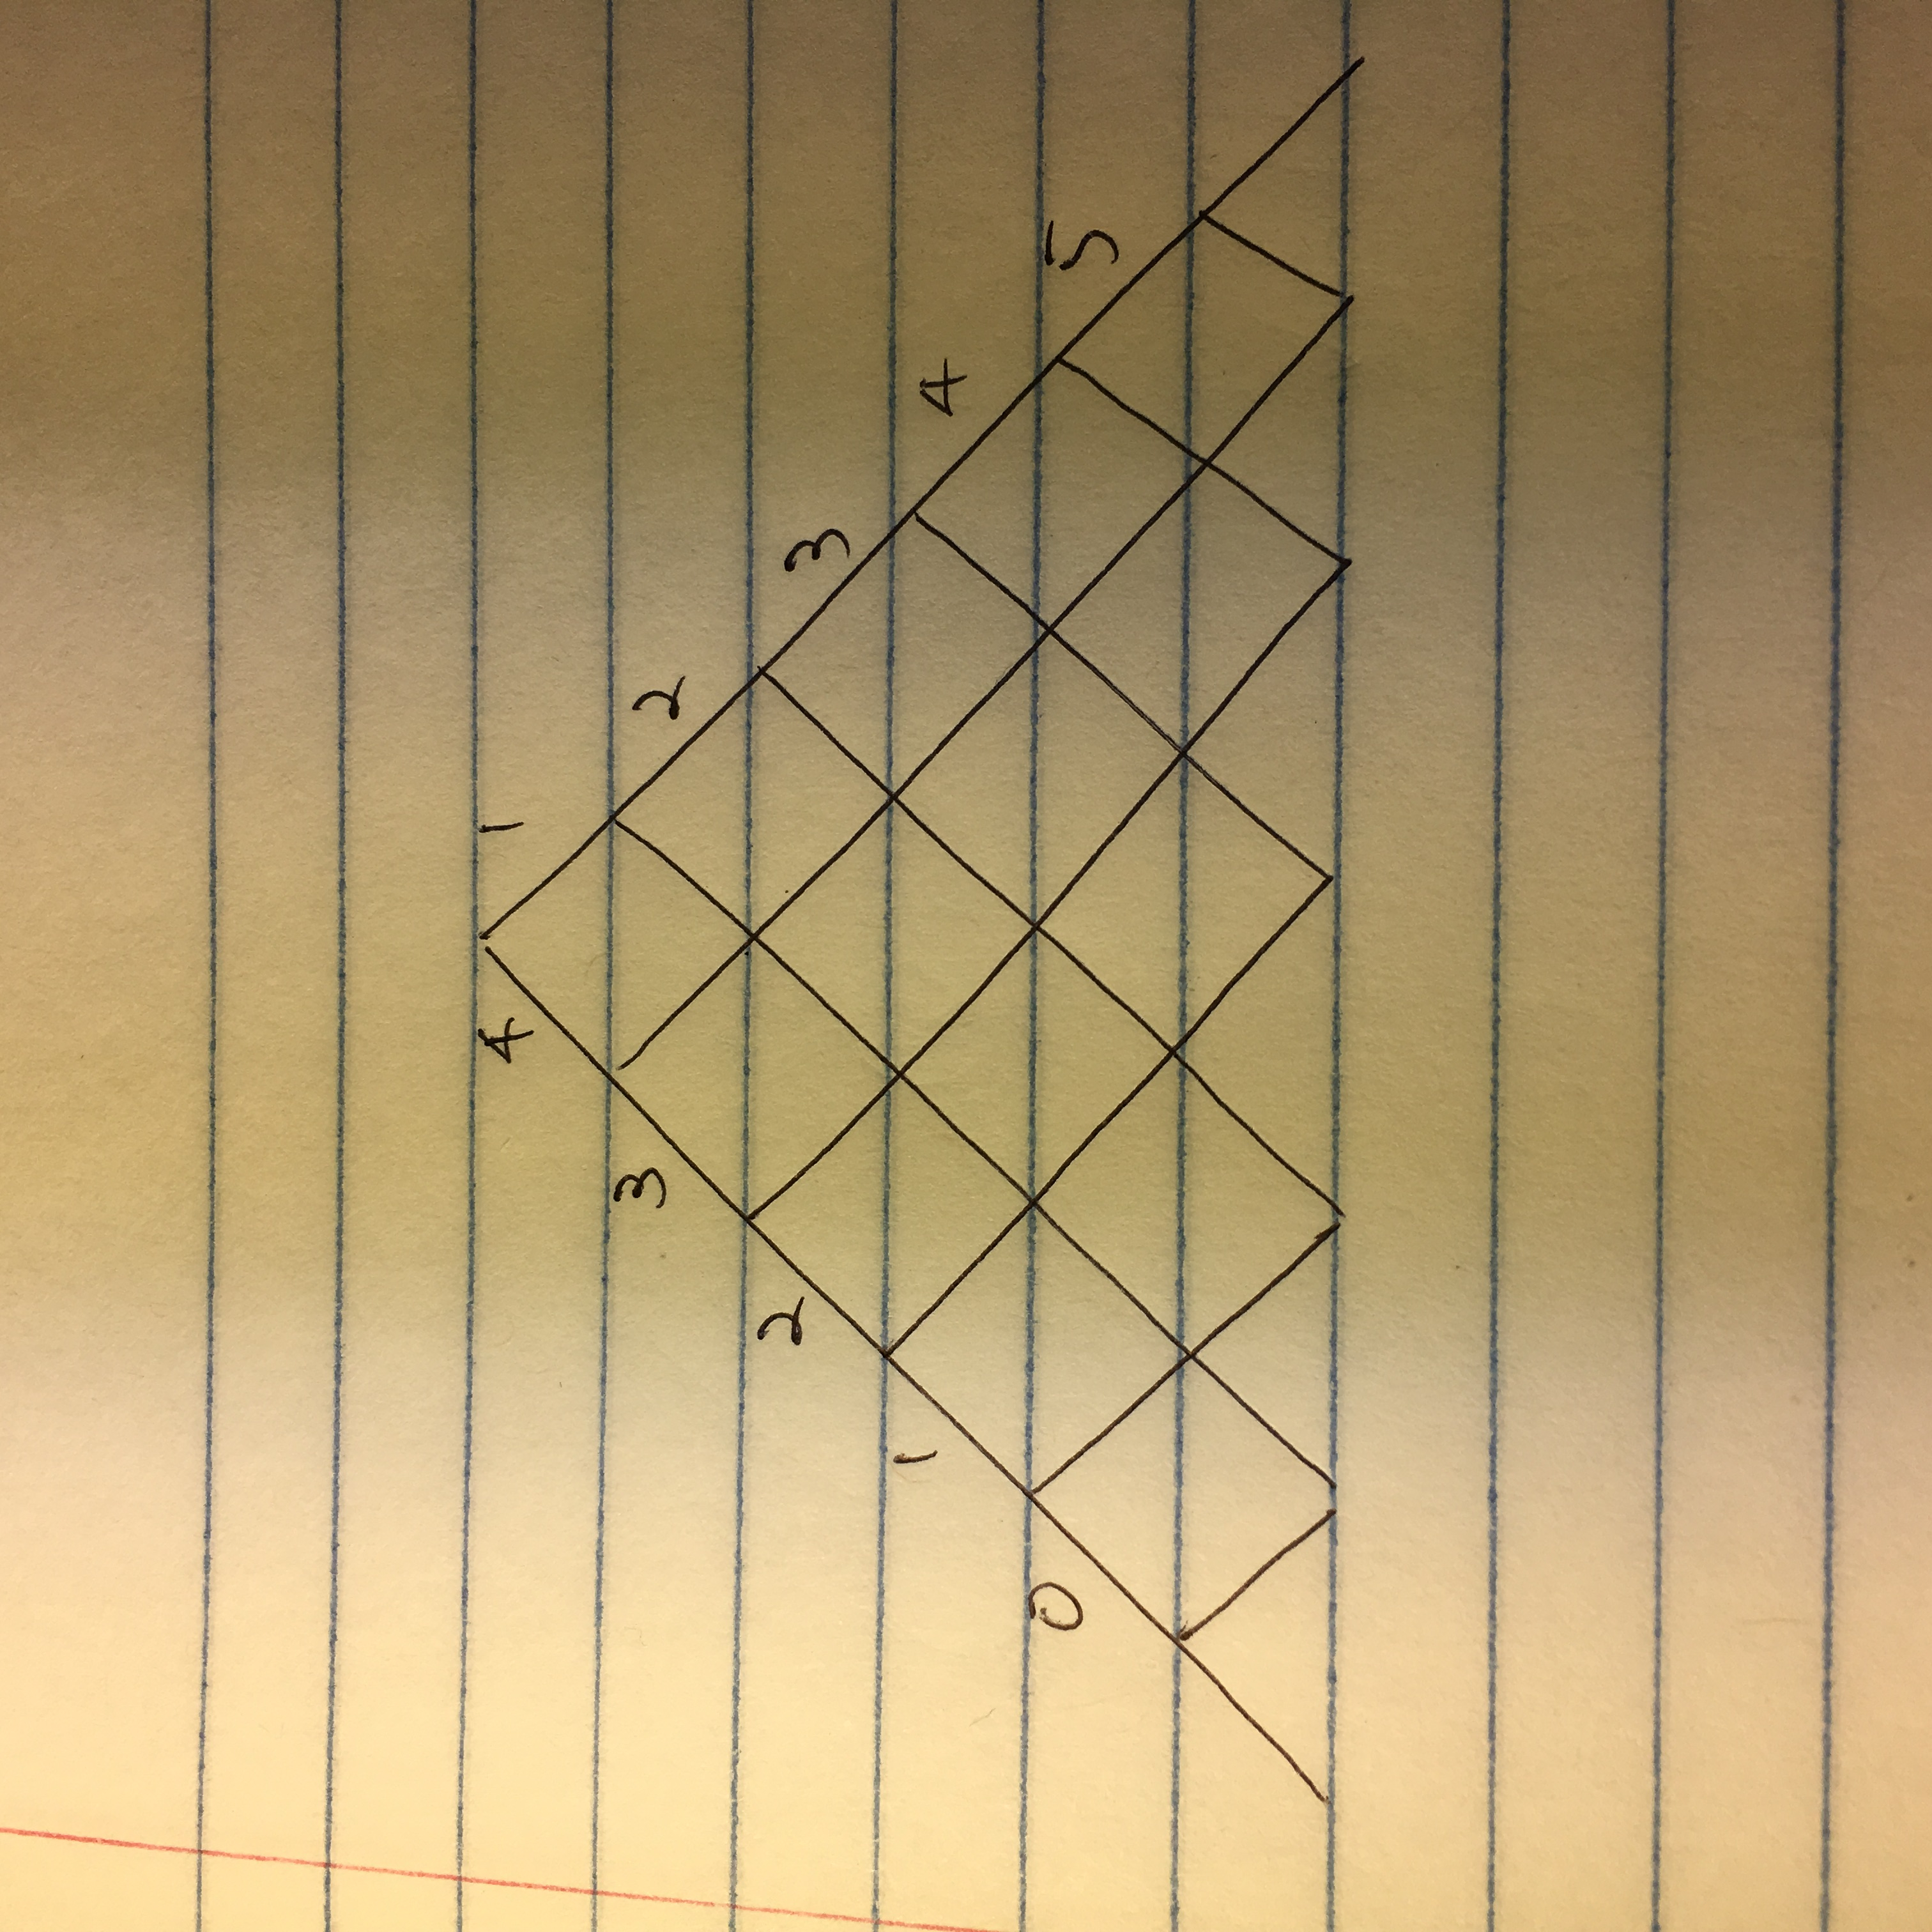
\includegraphics[scale=0.04]{figure2.jpg}
	\caption{Tilted Table}
\end{figure}

In this table, I will store the root of the subtree, and the number of the total node without the root.

This table matrix will be denoted as $e[i,j]$.

\[
  e[i,j] = \left.
  \begin{cases}
    0 &  j=i-1 \\
    2 &  j=i \\
    e[i,r]+e[r+1,j]  & \text{for possible }  r \in [i,j-1] \\
  \end{cases}
  \right\} 
\]
Note that $r$ is only possible if $e[i,r]$ is in range of $e[r+1,j]$ / 3, $e[r+1,j]$ * 3.
If $r$ is possible, then make the smaller number tree the subtree of the bigger number tree's root.
Also, store a root for $e[i,j]$. That is, if the root is $k_r$ for $e[i,j]$, store that root.

Following is how I add two tree.
\begin{figure}[hbt]
	\centering
	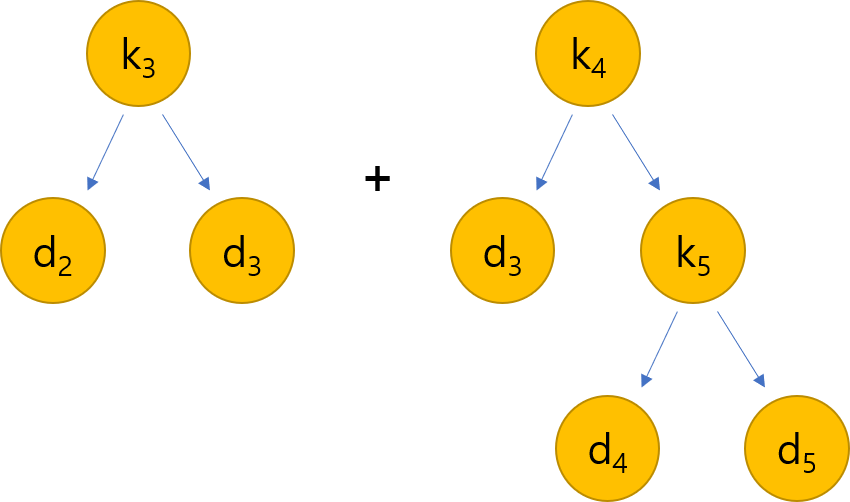
\includegraphics[scale=0.4]{figure3.png}
	\caption{Adding Two Tree}
\end{figure}

The total number of node except the root is 2 for left tree, and 4 for right tree. This does not violate the range. So the smaller number tree becomes the subtree of the larger number tree. Following is the result.

\begin{figure}[hbt]
	\centering
	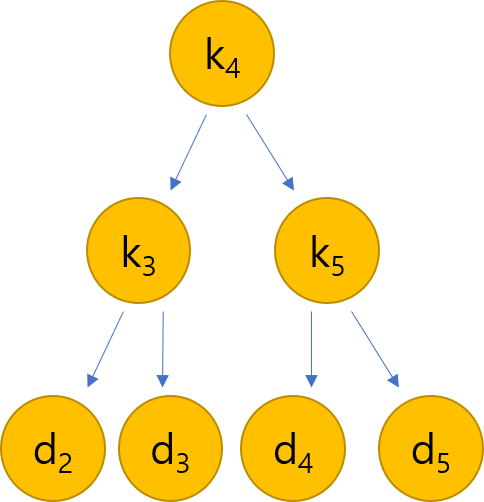
\includegraphics[scale=0.4]{figure4.png}
	\caption{Result Tree}
\end{figure}

\end{enumerate}


\end{document}
